\begin{figure}[h]		
	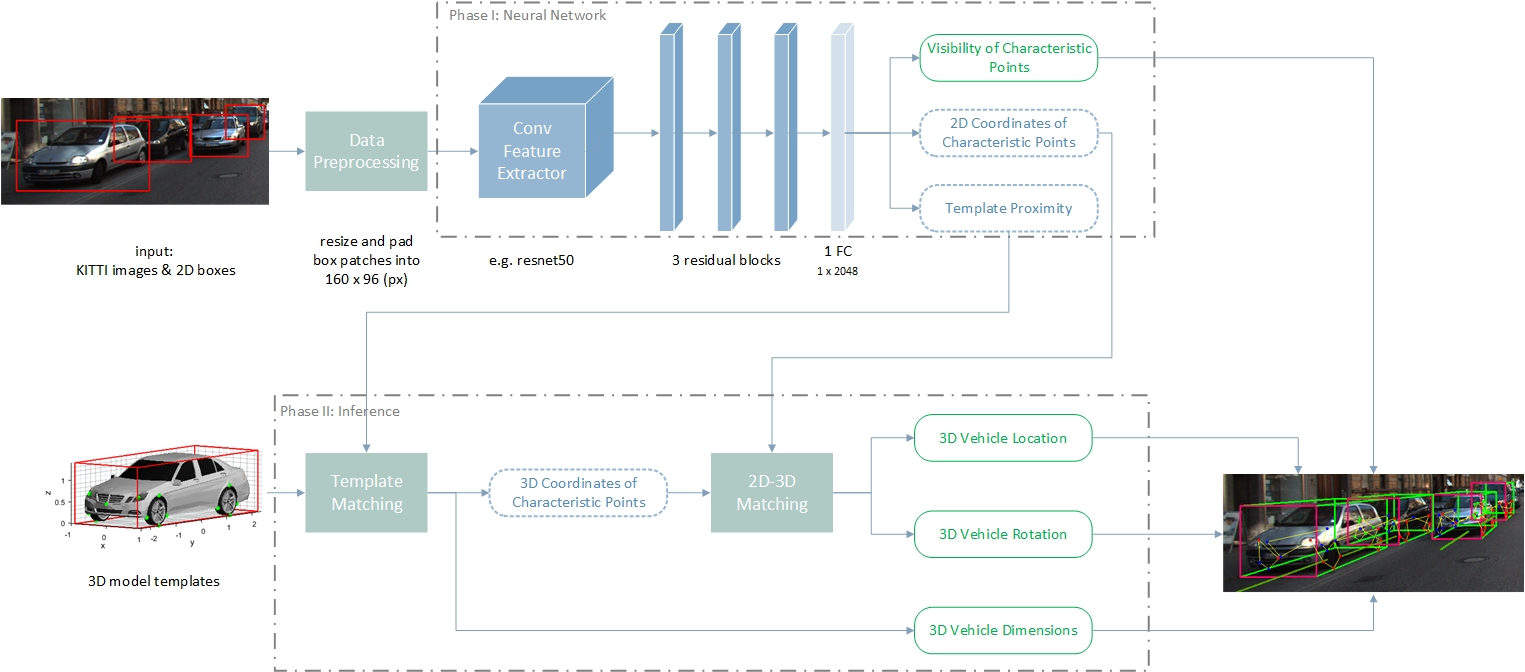
\includegraphics[width=1\textwidth]{app_archi_box_0522.jpg}
	\caption{The Architecture of our Approach}
	\centering
	\label{figure:app_archi}
\end{figure}

In this section, we elaborate our approach for 3D pose estimation of vehicles in monocular images. Our approach is based on 2D vehicle detection, \ie the 2D bounding boxes of vehicles are given as prior, since 2D object detection techniques, such as YOLO \cite{DBLP:journals/corr/RedmonF16}, Faster R-CNN \cite{DBLP:journals/corr/RenHG015}, SSD \cite{DBLP:journals/corr/LiuAESR15}, R-FCN \cite{DBLP:journals/corr/DaiLHS16}, and FPN \cite{DBLP:journals/corr/LinDGHHB16},  have achieve very high accuracy while  end-to-end 3D object detection performance is still primitive.  The overall architecture of the approach is illustrated in Figure \ref{figure:app_archi}. It consists of two main phases. The first one is the CVT Network which takes the KITTI images and the 2D bounding box as inputs and predicts the visibility property and 2D coordinates of all characteristic points, as well as the template proximity. The details are presented in section \ref{network}.  The other phase estimates the 3D location, rotation, and dimension of each vehicle based on the 3D vehicle dataset and the outputs of the CVT Network. Section \ref{inference} demonstrated this phase in detail. The KITTI dataset and the 3D vehicle dataset are described in section \ref{data}.


